\documentclass[conference]{IEEEtran}
\IEEEoverridecommandlockouts
% The preceding line is only needed to identify funding in the first
% footnote. If that is unneeded, please comment it out.

\usepackage{booktabs}
\usepackage{cite}
\usepackage{url}
\usepackage{multirow}
\usepackage{pgfplots}
\usepackage{tikz}
\usetikzlibrary{matrix,fit,shapes,calc,positioning,shadows,arrows,shapes,backgrounds,decorations.markings,fadings}
\usepackage{listings}
\usepackage[caption=false, font=footnotesize]{subfig}
%%%%%%%%%%%%% code listing
\renewcommand{\ttdefault}{pcr}
\lstset{
  basicstyle=\scriptsize\ttfamily,
  keywordstyle=\scriptsize\ttfamily\bfseries,
  language=C,             % choose the language of the code
  frame=single,              % adds a frame around the code
  aboveskip=0pt,
  belowskip=0pt,
  breaklines=true,           % sets automatic line breaking
  breakatwhitespace=false,   % sets if automatic breaks should only happen at
  showspaces=false,
  %numbersep=5pt,              % Abstand der Nummern zum Text
  %tabsize=2,                  % Groesse von Tabs
  %extendedchars=true,         %
  %breaklines=true,            % Zeilen werden Umgebrochen
  keywords=[2]{tcp, flag, threshold, track, count, seconds, classtype, sid}
}
\usepackage{balance}
\usepackage{wrapfig}
\usepackage{enumitem}
\usepackage{color, colortbl}
\definecolor{Gray}{gray}{0.9}

\newcommand{\tname}{\textsc{Syrius}} %% name of the technique
\newcommand{\ie}{i.e.}
\newcommand{\eg}{e.g.}
\newcommand{\aka}{a.k.a.}
\newcommand{\etal}{and colleagues}
\newcommand{\nids}{NIDS}
\newcommand{\metas}{Metasploit}
\newcommand{\suri}{Suricata}
\newcommand{\numrulessuri}{27.8K}
\newcommand{\percRulesWithContent}{93.5\%}
\newcommand{\numundetected}{\Fix{XX\%}}
\newcommand{\CodeIn}[1]{{\small{\texttt{#1}}}}
\newcommand{\MyComment}[1]{}

%% review
\newcommand{\Fix}[1]{{\textbf{[[}\color{magenta}#1}\textbf{]]}}
\newcommand{\Mar}[1]{{\textbf{[[Marcelo:~}\color{red}#1}\textbf{]]}}
\newcommand{\Luc}[1]{{\textbf{[[Lucas:~}\color{blue}#1}\textbf{]]}}
\newcommand{\Gui}[1]{{\textbf{[[Guilherme:~}\color{green}#1}\textbf{]]}}

\def\denseitems{
   \itemsep1pt plus1pt minus1pt
   \parsep0pt plus0pt
   \parskip0pt\topsep0pt}

%% numbers
\newcommand{\totoptions}{162}
\newcommand{\numproto}{11}
\newcommand{\totoptionsrelevant}{153}



%% \usepackage{cite}
%% \usepackage{amsmath,amssymb,amsfonts}
%% \usepackage{algorithmic}
%% \usepackage{graphicx}
%% \usepackage{textcomp}
%% \usepackage{xcolor}

\def\BibTeX{{\rm B\kern-.05em{\sc i\kern-.025em b}\kern-.08em
    T\kern-.1667em\lower.7ex\hbox{E}\kern-.125emX}}
\begin{document}

\title{Search-based Synthesis of Network Intrusion Detection Rules}

%%%%%%%%%%% Anonymized

%% \author{\IEEEauthorblockN{1\textsuperscript{st} Given Name Surname}
%% \IEEEauthorblockA{\textit{dept. name of organization (of Aff.)} \\
%% \textit{name of organization (of Aff.)}\\
%% City, Country \\
%% email address}
%% \and
%% \IEEEauthorblockN{2\textsuperscript{nd} Given Name Surname}
%% \IEEEauthorblockA{\textit{dept. name of organization (of Aff.)} \\
%% \textit{name of organization (of Aff.)}\\
%% City, Country \\
%% email address}
%% \and
%% \IEEEauthorblockN{3\textsuperscript{rd} Given Name Surname}
%% \IEEEauthorblockA{\textit{dept. name of organization (of Aff.)} \\
%% \textit{name of organization (of Aff.)}\\
%% City, Country \\
%% email address}
%% \and
%% \IEEEauthorblockN{4\textsuperscript{th} Given Name Surname}
%% \IEEEauthorblockA{\textit{dept. name of organization (of Aff.)} \\
%% \textit{name of organization (of Aff.)}\\
%% City, Country \\
%% email address}
%% \and
%% \IEEEauthorblockN{5\textsuperscript{th} Given Name Surname}
%% \IEEEauthorblockA{\textit{dept. name of organization (of Aff.)} \\
%% \textit{name of organization (of Aff.)}\\
%% City, Country \\
%% email address}
%% \and
%% \IEEEauthorblockN{6\textsuperscript{th} Given Name Surname}
%% \IEEEauthorblockA{\textit{dept. name of organization (of Aff.)} \\
%% \textit{name of organization (of Aff.)}\\
%% City, Country \\
%% email address}
%% }

\maketitle

\begin{abstract}
...
\end{abstract}

\begin{IEEEkeywords}
NIDS, synthesis, search
\end{IEEEkeywords}

\section{Introduction}

Network Intrusion Detection Systems (\nids{}) are software systems
that monitor the network traffic for malicious behavior and act
accordingly by blocking messages or alerting humans about suspicious
events~\cite{Mitchell:2014:SID:2597757.2542049}. \nids{} are typically
placed behind a firewall, vetting the traffic that the firewall did
not block. Various open-source (\eg{}, Snort~\cite{snort} and
Suricata~\cite{suricata}) and commercial implementations (\eg{},
SolarWinds~\cite{solarwinds} and IBM QRadar~\cite{qradar}) exist
today. These systems are very popular in industry to secure local
computer networks given the amount of potential malicious traffic that
exist on the Internet today.

\sloppy \nids{} are typically categorized in two
groups~\cite{kumar2007survey}: 1)~rule-based and 2)~anomaly-based. A
rule-based \nids{} (\aka\ signature-based NIDS) checks if the network
traffic matches a fixed set of
rules. Figure~\ref{fig:synflood-example} shows an example rule of
Suricata~\cite{suricata}, a popular open-source \nids{}. This rule
prescribes a method to capture SYN flood attacks to a
server~\cite{Douligeris:2004:DAD:987153.987158} that can result in
denial of service. Rule-based \nids{} focuses on known attacks whereas
anomaly-based \nids{} focuses on unanticipated attacks that could be
observed through suspicious network
traffic~\cite{kumar2007survey,Mitchell:2014:SID:2597757.2542049,cordy-etal-issta19}.

Rule-based and Anomaly-based NIDS are complementary. This paper
proposes a technique, dubbed \tname{}, to automatically synthesize
rules from positive and negative examples (\ie{}, benign and malicious
traffic). The main scenario of application is one where an
anomaly-based NIDS identifies abnormal traffic and signals that
traffic to \tname{} to craft rules that can be used by rule-based
NIDS. The core motivation is that attackers are productive in creating
new ways to circumvent existing protections and manual creation of
rules is tedious and time-consuming.\Mar{Lucas/Guilherme: (IMP) do we
  have data to support this?} For those reasons, synthesizing rules to
circumvent those issues is an important problem.

\Fix{summarize how the technique works}

\Fix{summarize results}

This paper makes the following contributions. \Fix{...}

\section{Illustrative Example}
\label{sec:suri-metas-coverage}

This section 1) shows an example rule of Suricata and briefly explains
the format of Suricata rules, 2) presents an example of
a network attack, and 3) illustrates how \tname{} performs to
synthesize the rule that would capture the attack.

\subsection{Suricata Rules}
\label{sec:example-suricata-rules}

\Mar{Lucas/Guilherme, verifique se isto esta correto}
Figure~\ref{fig:synflood-example} shows an example rule of
Suricata~\cite{suricata}, a popular open-source \nids{} maintained by
the Open Information Security Foundation (OISF)~\cite{oisf}. A
Suricata rule is divided in three parts---action, header, and rule
options~\cite{suri-rule-format}. The action part appears as the first
word in the rule description. In this case, \CodeIn{alert}. An action
denotes the task that needs to be executed if the rule pattern is
satisfied. In this case, a message will be sent to sys admins if the
rule pattern is satisfied. Other options of actions include pass,
drop, and reject. The header comes after the action in the rule
description. It restricts the information flow covered by the
rule. For this rule, the header is \CodeIn{tcp \$HOME\_NET any ->
  \$EXTERNAL\_NET any}, which instructs Suricata to inspect
\CodeIn{tcp} traffic flowing from any port in the home network to any
other address outside the home network. The variables
\CodeIn{\$HOME\_NET} and \CodeIn{\$EXTERNAL\_NET} are
configurable. The rule options come after the header. It is a
semi-colon-separated sequence of properties\Mar{should we call it an
  option or property?}, where each property is a key-value pair
describing a distinct characteristic of the attack.

\subsection{SYN Flood Attack}

The SYN Flood attack exploits a vulnerability in the TCP/IP handshake
to establish a TCP connection~\cite{cloudfare-synflood}. The handshake
works as follows. First, a client sends a SYN packet to the server,
requesting a connection. Second, the server responds with a SYN-ACK
packet to the client. Third, the client responds with an ACK message
and the connection is established. Aware of the protocol, an attacker
sends multiple SYN packets to different ports of a server, often using
fake IP addresses. Without proper protection, the server accepts the
connection requests and eventually legitimate connection requests
cannot be satisfied due to resource exhaustion.

Figure~\ref{fig:synflood-example} shows a Suricata rule to capture
this attack. The critical parts are the option \CodeIn{flags: S,12},
which identifies a SYN packet and the option \CodeIn{threshold: type
  both, track by\_dst, count 5000, seconds 5}, indicating that a high
volume of such packets should be requested in a short period of time.

\begin{figure}[t]
  \lstinputlisting[language=C,numbers=none]{synflood.suricata}
  \caption{Suricata rule for SYN Flood Attacks.\Mar{colocar
      propriedades em negrito}}
  \label{fig:synflood-example}
\end{figure}

\subsection{\tname\ on SYN Flood Attack}

\Mar{Guilherme/Lucas (CRI): we need to show how \tname{} works on this
  example. What is the input? How long does it take to generate the
  rule? Is the rule generate exactly the same?}

\section{Approach}

\tname{} is a search-based approach that uses positive and negative
network traffic examples to synthesize signature-based NIDS rules,
such as those from Snort and Suricata. \tname{} synthesizes rules in
two steps. First, it produces a potentially overspecified rule that
captures the negative example that is provided as input. Then, it uses
positive examples to eliminate unnecessary options from the rule. The
goal of \tname\ is to create a rule that captures only the negative traffic.

\subsection{Problem Characterization}

One important step in search-based optimization is to characterize a
candidate solution to the target problem. Candidate solutions are the
objects that the search optimize towards solutions. In this case, a a
candidate solution is an encoding of a Suricata rule.  \tname\ encodes
the rule options segment of a Suricata rule (see
Section~\ref{sec:example-suricata-rules}) as a vector of Option
objects. Some options are discarded as they only serve for
documentation. For example, the options \CodeIn{msg},
\CodeIn{classtype}, and \CodeIn{misc-activity}, appearing in the
example on Figure~\ref{fig:synflood-example}, have no influence in
triggering the actions associated with rules. The option
\CodeIn{flags}, however, is relevant to trigger the action. \tname{}
models that option with a data structure storing two fields, one of
character type and another of integer type. This enables \tname{} to
mutate each element separately. Similar encodings are used in modeling
the other relevant options. We found what is (ir)relevant by
inspecting Suricata code for the presence of \CodeIn{eval} functions,
which are invoked from a main look to process every Suricata rule. The
presence of such a function for a given option indicates that it is
relevant for triggering some action of some rule.

Options can be specific to a given protocol or general and they can be
influential on triggering an action or
not. Figure~\ref{fig:distribution-rules-protocol} shows the
distributions of these options per protocol and their relevance for
triggering rule actions.

\pgfplotsset{width=5.5cm,compat=1.8}
\begin{figure}[h!]
  \centering
  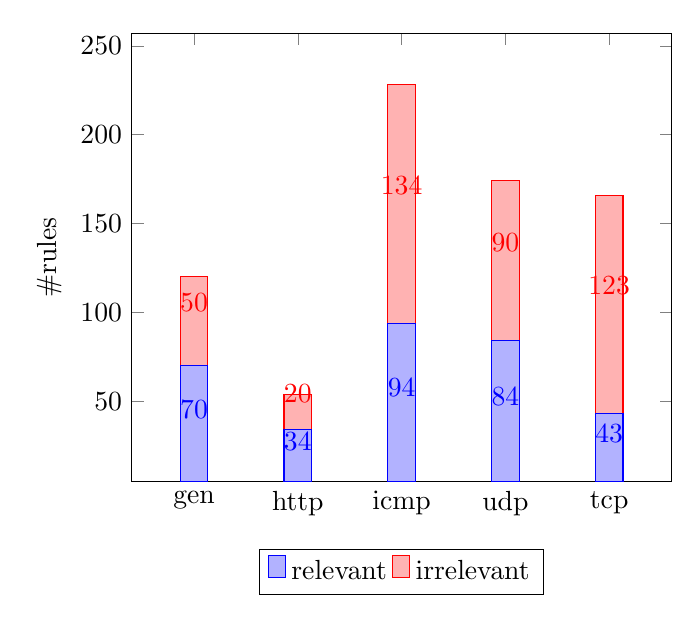
\begin{tikzpicture}
    \begin{axis}[
        ybar stacked,
        enlargelimits=0.15,
        legend style={at={(0.5,-0.15)},
          anchor=north,legend columns=-1},
        ylabel={\#rules},
        symbolic x coords={gen, http, icmp, udp, tcp},
        xtick=data,
        nodes near coords,
        nodes near coords align={vertical},
      ]
      \addplot coordinates {(gen,70) (http,34) (icmp,94) (udp,84) (tcp,43)};
      \addplot coordinates {(gen,50) (http,20) (icmp,134) (udp,90) (tcp,123)};    
      \legend{relevant, irrelevant}
    \end{axis}
  \end{tikzpicture}
  \caption{\label{fig:distribution-rules-protocol}Distribution of
    rules per protocol and relevance for triggering action.}
\end{figure}

\subsection{Initial State}

To bootstrap the search, \tname{} needs to select an initial
solution. When creating such candidate solution, \tname{} first looks
for the protocol related to the malicious input traffic. Then, it
selects the relevant options for that protocol and initializes the
option vector with default values. \Mar{Suricata define valores
  default?  Vcs. definiram?  Isto foi baseado em popularidade ou o
  que?}

%% \tname{}
%% uses an abstract representation of a Suricata rule that reflects the
%% concrete representation of the rule. The concrete rule representation
%% is the one actually used by Suricata whereas the abstract
%% representation is the one \tname{} uses to run the search.

\subsection{Fitness Functions}

The fitness value of a candidate solution $c$, modeling the rule
options $o_1, \dots, o_n$ is given by $f(c)=1-\Sigma{d(o_i,m)}/n$,
where $i$ ranges from 1 to $n$ and $m$ denotes the negative
traffic. The higher the fitness value the better, \ie{}, the fitter
the candidate solution $c$ will be.  The value of the expression
$d(o_i,m)$, associated with option $o_i$, ranges over
0-1. Consequently, the value of the expression $\Sigma{d(o_i,m)}/n$
itself is in the 0-1 range, as there are $n$ options, and the range of
the function is 0-1.

As usual, we used customized distance functions to compute $d(o_i,
m)$. For example, let us consider the \CodeIn{flags} option, discussed
on Figure~\ref{fig:synflood-example}. Recall that this option
identifies the SYN packet in the tcp protocol and that its encoding in
\tname{} stores two attributes---one categorical and one
numerical. The value of $d(o_i, m)$, in this case, is obtained by
computing the normalized Euclidean distance in the two-dimensional
space. Considering that each of the two dimensions has cardinality of
ten, the distance of a candidate solution holding the option
\CodeIn{flags(S,13)} to the solution will be 0.22
(=$1/\sqrt{20}$). Note that the smaller the distance the better.

\tname{} uses a modified version of Suricata to measure distance. It
updates the rule set that the modified version of Suricata analyses,
injects the traffic on the network, and monitors the execution. Each
rule option has an associated \CodeIn{eval} function in code. \tname{}
monitors the execution of these functions to identify how far it is
from returning true, which indicates it is closer to trigger the
action associated with the rule. For the example above,
\Fix{Lucas/Guilherme, it would be good to show how this looks like in
  code}

\subsection{Search}

\tname{} is a single-individual hill-climbing like search.

\section{Evaluation}

\Mar{Lucas/Guilherme (CRI): precisamos dar pontape inicial propondo
  perguntas de pesquisa. Eu faco ajustes em seguida.}

\section{Threats to Validity}

External Validity. \Fix{elaborate ...how popular are Suricata/Metasploit?}

\section{Related Work}

\Fix{...}

\balance
%\vspace*{-2\baselineskip}
\bibliographystyle{IEEEtran}
\bibliography{references}

\end{document}

%%  LocalWords:  Suricata SolarWinds QRadar NIDS OISF TCP ACK msg tcp
%%  LocalWords:  encodings eval cardinality
